\section{The problem and the principal results}\label{sec:results}

Repeated rounding is a simple deterministic operation with unexpectedly
structured large-scale behavior. Fix a real number $m>0$ and an integer
$n\geq0$. Define
\begin{equation}\label{eq:forward}
 x_1=n,\qquad
 x_k=k^m\floor{\frac{x_{k-1}}{k^m}}\quad(k\geq2),\qquad
 \tau_m(n)=\min\{k\geq1:x_k=0\}.
\end{equation}
The value $x_k$ is nonnegative and does not increase with $k$. The stopping
time is finite: once $k^m>n$, the next rounding gives zero. We use the
convention $\tau_m(0)=1$. For $n>0$, one always has $\tau_m(n)\geq2$.
When $m$ is not an integer, the intermediate values can be real; the
quotient $x_k/k^m$ is nevertheless an integer for every $k\geq2$.

The sequences for $m=1,2,3$ are respectively \OEIS{A073047},
\OEIS{A082527}, and \OEIS{A082528}. Cloitre's entry for the cubic case also
asks for the asymptotic law for every real $m>0$~\cite{oeis-linear,oeis-square,oeis-cube}.
The following theorem determines that law and its constant.

\begin{theorem}[Power-rounding extinction]\label{thm:main}
For every fixed real $m>0$, set
\begin{equation}\label{eq:constants}
 c_m=m\,\Gamma\!\left(\frac{m}{m+1}\right)^{m+1},\qquad
 L_m=\frac1{c_m}.
\end{equation}
Then, as the integer $n$ tends to infinity,
\begin{equation}\label{eq:main}
 \tau_m(n)\asym(c_m n)^{1/(m+1)}.
\end{equation}
Equivalently, if $T_m(K)$ is the smallest integer initial value that
survives through stage $K$, then
\begin{equation}\label{eq:threshold-main}
 T_m(K)\asym L_m K^{m+1}.
\end{equation}
\end{theorem}

In particular,
\begin{align}
 \tau_2(n)&\asym
 \left(2\Gamma(2/3)^3n\right)^{1/3},\label{eq:square}\\
 \tau_3(n)&\asym
 \left(3\Gamma(3/4)^4n\right)^{1/4}.\label{eq:cube}
\end{align}
The constants are
\begin{equation}\label{eq:decimals}
 c_2=4.965917162430455473\ldots,\qquad
 c_3=6.764822981008760234\ldots.
\end{equation}
These identify the values $4.96\ldots$ and $6.76\ldots$ conjectured
numerically in the two OEIS entries. The specialization $c_1=\pi$ is the
classical Tchoukaillon constant, whose prior history is discussed in
\cref{sec:history}.

The same proof identifies more than a stopping index. Define the crossing
times
\begin{equation}\label{eq:crossing-def}
 t_0=1,\qquad
 t_j=\prod_{r=1}^{j}\left(1-\frac1{(m+1)r}\right)\quad(j\geq1),
\end{equation}
and the continuous function $y_m:(0,1]\to[0,\infty)$ by
\begin{equation}\label{eq:profile-def}
 y_m(t)=\frac{(m+1)j-1}{m}\,t_{j-1}-jt,
 \qquad t_j\leq t\leq t_{j-1}.
\end{equation}
The definitions agree at each shared endpoint. Set
\begin{equation}\label{eq:mass-profile}
 F_m(t)=c_m t^m y_m(t)\quad(0<t\leq1),\qquad F_m(0)=1.
\end{equation}

\begin{theorem}[The full extinction trajectory]\label{thm:forward-profile}
Let $J=\tau_m(n)$ for $n>0$, and put
\[
 X_n(t)=\frac{x_{\max(1,\lfloor Jt\rfloor)}}n,
 \qquad 0\leq t\leq1.
\]
Then
\begin{equation}\label{eq:uniform-forward}
 \sup_{0\leq t\leq1}|X_n(t)-F_m(t)|\longrightarrow0.
\end{equation}
Thus the fraction of the initial value remaining, plotted against the
fraction of the extinction time elapsed, has an explicit deterministic
limiting shape.
\end{theorem}

Our extension to more general weights uses a local condition on their
successive ratios. This condition is stronger than specifying only their
leading growth.

\begin{theorem}[Smooth-weight universality]\label{thm:weights-main}
Suppose $w_1=1$, $w_k>0$, and
\begin{equation}\label{eq:smooth-weights}
 k\left(\frac{w_k}{w_{k-1}}-1\right)\longrightarrow m>0.
\end{equation}
Replace $k^m$ in \cref{eq:forward} by $w_k$, and denote the corresponding
threshold and stopping time by $T_w(K)$ and $\tau_w(n)$. Then
\begin{equation}\label{eq:weights-main}
 T_w(K)\asym L_m K w_K,\qquad
 L_m\tau_w(n)w_{\tau_w(n)}\asym n.
\end{equation}
With $J=\tau_w(n)$, the normalized forward trajectory converges uniformly
to the same $F_m$ in \cref{eq:mass-profile}.
\end{theorem}

Theorem~\ref{thm:weights-main} allows logarithmic factors, shifts, and many
small perturbations. Its hypothesis cannot simply be replaced by ordinary
regular variation: \cref{sec:clock} constructs weights
$w_k\asym(k/r)^m$ for which the threshold constant is $L_m/r$.

\subsection{What has and has not been resolved}

\begin{center}
\small
\begin{tabular}{@{}p{.28\linewidth}p{.64\linewidth}@{}}
\toprule
Question or claim & Status in this report\\
\midrule
A082528, every real $m>0$ & The stated leading-equivalence conjecture is proved; $c_m$ is explicit.\\[3pt]
A082527 and A082528 constants & The square and cube constants are determined by \cref{eq:square,eq:cube}.\\[3pt]
A073047 leading equivalent & Recovered as a classical specialization, with no novelty claim.\\[3pt]
A073047 bounded error & The stronger assertion $\tau_1(n)=\sqrt{\pi n}+O(1)$ is not proved here.\\[3pt]
Full trajectories and smooth weights & Proved in \cref{thm:forward-profile,thm:weights-main}.\\[3pt]
Quantitative discrete errors & No rate is inferred from the compactness argument; these are explicit research questions.\\[3pt]
Historical priority & No matching general power theorem was found in the targeted source search; exhaustive priority is not certified.\\
\bottomrule
\end{tabular}
\end{center}

All limits involving $m$ in the first three theorems hold for fixed $m>0$.
They make no assertion uniform in a moving parameter $m=m(n)$.

\section{Historical context and the ProveIt starting point}\label{sec:history}

\subsection{The OEIS questions}

Cloitre introduced the square and cube stopping sequences in April 2003.
The entry for A082528 explicitly asks whether the first zero for real
powers $k^m$ has order $(c(m)n)^{1/(m+1)}$. A082527 records the numerical
constant $4.96\ldots$, and A082528 records $6.76\ldots$
\cite{oeis-square,oeis-cube}. The entries were inspected during the source
audit for this report. Their shared site-footer time is not treated as an
individual sequence revision date.

The square entry contains a minor arithmetic slip in its example for
$n=10$: the correct intermediate value is
$4\lfloor10/4\rfloor=8$. The reported stopping index $3$ is correct.
The definitions, programs, and initial terms agree with
\cref{eq:forward}; the slip has no effect on the theorem.

\subsection{The classical linear sieve}

When $m=1$, the backward threshold is A002491. Starting with $K$, one
successively rounds upward to a multiple of $K-1,K-2,\ldots,1$. Its first
values are
\[
 1,2,4,6,10,12,18,22,30,34,\ldots.
\]
This is a standard description of the Tchoukaillon or Mancala sieve
\cite{oeis-threshold}. Erd\H{o}s and Jabotinsky proved
\begin{equation}\label{eq:classical-error}
 T_1(K)=\frac{K^2}{\pi}+O(K^{4/3})
\end{equation}
and proposed the sharper $O(K)$ error~\cite{erdos-jabotinsky}.
Their paper already analyzes successive ranges of equal integer
increments. The use of such ranges and a product limit in the present
proof belongs to that established method.

There is a relevant caution about error terms. Broline and Loeb later
claimed the sharper threshold estimate~\cite{broline-loeb}. Knuth's 2021
comment recorded in A002491 identifies an accumulation-of-errors problem
in that argument and explains why its stated estimates do not establish
the claimed improvement~\cite{oeis-threshold}. We use neither that
sharpening nor any consequence of it. The classical
\cref{eq:classical-error} would imply
\[
 \tau_1(n)=\sqrt{\pi n}+O(n^{1/6}),
\]
whereas the $O(1)$ error recorded as presumptive in A073047 is a stronger
assertion.

Brown's exposition obtains the ordinary constant from successive
parabolic pieces and a Wallis product~\cite{brown}. A 2023 answer by
Thomas Leh\'ericy studies a different generalization, rounding upward to
the $r$th admissible multiple, and obtains a ratio of Gamma
functions~\cite{lehericy}. Its use of fixed increment regimes and a final
truncation estimate is methodologically relevant. Its parameter changes
the rounding rule; the parameter $m$ here changes the moduli themselves.
The two statements concern different recurrences.

We also checked Li's 2026 preprint on the two-dimensional Tchoukaillon
array~\cite{li}. Its main theorem concerns a uniform quadratic
approximation to array entries. It does not state the real-power
extinction theorem proved here. None of our proofs depends on that
preprint or on its discussion of sharp edge estimates.

\subsection{Repository audit and choice of target}

The research began with the current ProveIt repository~\cite{proveit}.
Targeted searches and directory inspection showed extensive recent
work on OEIS asymptotics, including Bell-scale growth, derivative
expansion supports, and balanced-word enumeration. Those established
results were taken into account when choosing a question with a clear
remaining mathematical claim.

The repository search was indexed at revision
\begin{center}
\small\texttt{ce37e13f4aa16819c87c3ccc611362d15758f2ac}.
\end{center}
Exact searches for A082527, A082528, A073047, A002491, and Tchoukaillon
returned no matching treatment. We also inspected the 59-entry
\texttt{oeis-sequence-asymptotics} directory and the 58-entry
\texttt{series-and-transseries} directory at that revision. This is a
bounded nonduplication check; it is not a claim to have read every file,
binary, branch, or historical version of the repository.

The present article extends the repository's research program through a
new target. It is mathematically self-contained and assumes none of its
unrefereed reports as a theorem. The substantive contribution claimed
here is the real-parameter power theorem, its explicit constant, and the
trajectory and weight extensions. The classical linear case and the
increment-regime method are credited to the preceding literature.

\section{Exact reversal: extinction as a survival threshold}\label{sec:duality}

The forward process has a floor at every step and an initial value that
changes with the question being asked. Fixing a terminal stage instead
gives a convenient triangular recurrence.

\begin{definition}[Backward quotient array]\label{def:backward}
For an integer $K\geq1$, define
\begin{equation}\label{eq:backward}
 q_K^{(K)}=1,\qquad
 q_{k-1}^{(K)}=\ceil{\left(\frac{k}{k-1}\right)^m q_k^{(K)}}
 \quad(2\leq k\leq K),
\end{equation}
and put $T_m(K)=q_1^{(K)}$. We suppress the superscript $K$ when the
terminal stage is fixed.
\end{definition}

\begin{lemma}[Survival duality]\label{lem:duality}
For every integer $n\geq0$ and $K\geq1$,
\begin{equation}\label{eq:duality}
 \tau_m(n)>K\quad\Longleftrightarrow\quad n\geq T_m(K).
\end{equation}
More generally, a value $k^m Q$ at stage $k\leq K$, with $Q$ a
nonnegative integer, survives through stage $K$ if and only if
$Q\geq q_k^{(K)}$.
\end{lemma}

\begin{proof}
At stage $K$, survival means a positive multiple of $K^m$, so its smallest
integer quotient is $1$. Suppose the least quotient that survives from
stage $k$ has been identified as $q_k$. An input $(k-1)^m Q$ produces an
output at least $k^m q_k$ exactly when
\[
 \floor{\frac{(k-1)^m Q}{k^m}}\geq q_k
 \quad\Longleftrightarrow\quad
 Q\geq\frac{k^m q_k}{(k-1)^m}.
\]
The least admissible integer $Q$ is the ceiling in
\cref{eq:backward}. Backward induction reaches stage $1$, where the
initial value $n$ is already an integer and $1^m=1$.
\end{proof}

\begin{corollary}[Exact inverse and strict increase]\label{cor:inverse}
The sequence $T_m(K)$ is strictly increasing and unbounded. For $n>0$,
\begin{equation}\label{eq:exact-inverse}
 \tau_m(n)=1+\max\{K\geq1:T_m(K)\leq n\}.
\end{equation}
Equivalently, $\tau_m(n)=J$ if and only if
$T_m(J-1)\leq n<T_m(J)$.
\end{corollary}

\begin{proof}
For terminal stage $K+1$, the quotient at stage $K$ is
$\lceil((K+1)/K)^m\rceil\geq2$, whereas it is $1$ for terminal stage
$K$. Every map $Q\mapsto\lceil aQ\rceil$ with $a>1$ is strictly
increasing on the integers. Reversing further therefore gives
$T_m(K+1)>T_m(K)$. Formula~\eqref{eq:exact-inverse} follows from
\cref{lem:duality}.
\end{proof}

\subsection{The two estimates that control all rounding errors}

Write
\begin{equation}\label{eq:ak}
 a_k=\left(\frac{k}{k-1}\right)^m-1
     =\frac{m}{k}+O_m(k^{-2}).
\end{equation}
Because $q_k$ is an integer,
\begin{equation}\label{eq:increment}
 q_{k-1}-q_k=\ceil{a_kq_k}\geq1.
\end{equation}
Consequently,
\begin{equation}\label{eq:positive-drift}
 q_k\geq K-k+1.
\end{equation}
The inequality remains significant after scaling, even though
$q_K/K\to0$.

Multiplying the ceiling inequality by $(k-1)^m$ gives the second estimate:
\begin{equation}\label{eq:weighted-error}
 0\leq (k-1)^m q_{k-1}-k^m q_k<(k-1)^m.
\end{equation}
Telescoping in either direction yields
\begin{align}
 0&\leq T_m(K)-k^m q_k<\sum_{j=1}^{k-1}j^m,
       \qquad (k\geq2),\label{eq:small-tail}\\
 k^m q_k&\leq K^m+\sum_{j=k}^{K-1}j^m
        \leq K^m+\frac{K^{m+1}}{m+1}.
        \label{eq:global-bound}
\end{align}
For $k=1$, the difference in \cref{eq:small-tail} is exactly zero.
The last inequality follows by comparing the increasing function $x^m$
with its integral over $[1,K]$.

Equation~\eqref{eq:small-tail} is the key matching estimate: after a
macroscopic part of the backward trajectory has been computed, the
entire remaining part changes its weighted value by at most an explicit
sum. No assumption on the distribution of fractional parts is involved.

\begin{example}[A cubic threshold]
For $m=3$ and $K=4$, the backward quotients are
\[
 q_4=1,\qquad q_3=3,\qquad q_2=11,\qquad q_1=88.
\]
Thus $T_3(4)=88$. The initial value $88$ rounds through
$88,88,81,64,0$, so its stopping time is $5$. The value $87$ rounds
through $87,80,54,0$ and stops at $4$. This illustrates the strict
inequality $\tau_m(n)>K$ in the survival convention.
\end{example}

\section{A rigorous scaling limit for the backward array}\label{sec:limit}

For fixed $K$, define $y_K$ by linear interpolation through
\begin{equation}\label{eq:interpolation}
 y_K(k/K)=q_k^{(K)}/K,\qquad 1\leq k\leq K.
\end{equation}
Its domain is $[1/K,1]$. The limit will be considered on compact
subintervals of $(0,1]$; the singular endpoint $0$ is handled afterward
using \cref{eq:small-tail}.

\begin{lemma}[Compactness away from zero]\label{lem:compactness}
For every $0<\delta<1$, the restrictions of $y_K$ to $[\delta,1]$ are
uniformly bounded and uniformly Lipschitz for all sufficiently large
$K$. Every sequence of terminal stages tending to infinity has a
subsequence whose interpolants converge locally uniformly on $(0,1]$.
\end{lemma}

\begin{proof}
For $k\geq\delta K/2$, \cref{eq:global-bound} gives
\[
 \frac{q_k}{K}\leq
 \left(\frac{K}{k}\right)^m\left(\frac1K+\frac1{m+1}\right),
\]
which is bounded independently of $K$. On an interpolation interval
$((k-1)/K,k/K)$, its slope is
\begin{equation}\label{eq:slope}
 y_K'(t)=q_k-q_{k-1}=-\ceil{a_kq_k}.
\end{equation}
The expansion in \cref{eq:ak}, together with $q_k=O_\delta(K)$ and
$k\geq\delta K/2$, bounds this slope uniformly. The small enlargement to
$\delta/2$ handles the single grid interval containing $\delta$.
Arzel\`a--Ascoli on $[1/r,1]$, followed by a diagonal subsequence over
integers $r\geq2$, gives the stated compactness.
\end{proof}

\subsection{Selecting the nonzero terminal solution}

Let $y$ be any subsequential limit. Since $y_K(1)=1/K$,
\begin{equation}\label{eq:endpoint-limit}
 y(1)=0.
\end{equation}
Equation~\eqref{eq:increment} implies, including between grid points,
\begin{equation}\label{eq:limit-drift}
 y(s)-y(t)\geq t-s\qquad(0<s<t\leq1).
\end{equation}
In particular, $y(t)\geq1-t>0$ for $t<1$.

This is essential. If one wrote only
$y'=-\lceil my/t\rceil$ with $y(1)=0$, the identically zero function
would solve that terminal-value problem. The positive integer quotient
$q_K=1$ forces a drift of at least one at each reversed step and rules
out that spurious solution. We express this selection by the positive
ceiling
\begin{equation}\label{eq:positive-ceiling}
 C(u)=\max\{1,\lceil u\rceil\},\qquad u\geq0.
\end{equation}
For positive $u$, it is the ordinary ceiling.

\begin{lemma}[Passing through the ceiling discontinuities]\label{lem:ode}
Every subsequential limit is locally absolutely continuous and satisfies
\begin{equation}\label{eq:limit-ode}
 y'(t)=-C\!\left(\frac{my(t)}t\right)
 \quad\text{for almost every }t\in(0,1),
\end{equation}
together with \cref{eq:endpoint-limit,eq:limit-drift}.
\end{lemma}

\begin{proof}
Local Lipschitz continuity has already been proved. Define
$z(t)=my(t)/t$. For $0<s<t\leq1$, \cref{eq:limit-drift} gives
\[
 \frac{y(s)}s-\frac{y(t)}t
 \geq y(t)\left(\frac1s-\frac1t\right)+\frac{t-s}{s}>0.
\]
Thus $z$ is continuous and strictly decreasing as $t$ increases.
It is bounded on $[\delta,1]$, so it assumes an integer value at only
finitely many points in that interval.

Away from these exceptional points and $t=1$, let $k=\lceil Kt\rceil$.
The ratio expansion in \cref{eq:ak} and local uniform convergence show
\[
 a_kq_k\longrightarrow\frac{my(t)}t=z(t).
\]
The ceiling is continuous at the noninteger limit, so its value converges
to $C(z(t))$. Excluding also the countable union of grid points, \cref{eq:slope} therefore
converges to the claimed right-hand side. The slope bounds from
\cref{lem:compactness} permit dominated convergence in
\[
 y_K(t)=\frac1K-\int_t^1y_K'(s)\,ds.
\]
It follows that
\[
 y(t)=\int_t^1 C\!\left(\frac{my(s)}s\right)ds,
\]
which proves \cref{eq:limit-ode}.
\end{proof}

The argument does not assume uniform convergence of ceiling functions.
It proves convergence away from a finite exceptional set on each compact
interval and then uses an integrable uniform bound. That distinction is
what makes the limiting equation rigorous.

\subsection{Solving the increment regimes}

\begin{proposition}[Explicit profile and uniqueness]\label{prop:profile}
The function satisfying \cref{eq:endpoint-limit,eq:limit-drift,eq:limit-ode}
is unique. It is precisely $y_m$ in \cref{eq:profile-def}; consequently
\begin{equation}\label{eq:backward-convergence}
 y_K\longrightarrow y_m
 \quad\text{uniformly on every }[\delta,1],\quad\delta>0.
\end{equation}
\end{proposition}

\begin{proof}
The function $z(t)=my(t)/t$ decreases strictly from infinity to zero as
$t$ increases from zero to one. Its divergence at zero follows from
$y(t)\geq1-t$. Therefore every positive integer $j$ is attained at a
unique crossing time $t_j$.

On $(t_j,t_{j-1})$, one has $j-1<z(t)<j$ and hence $y'(t)=-j$.
Using $y(t_{j-1})=(j-1)t_{j-1}/m$ gives
\[
 y(t)=\frac{j-1}{m}t_{j-1}+j(t_{j-1}-t).
\]
At the next crossing, $y(t_j)=jt_j/m$, so
\[
 (m+1)j\,t_j=((m+1)j-1)t_{j-1}.
\]
This is exactly the product recurrence in \cref{eq:crossing-def}, and
the formula for $y$ is \cref{eq:profile-def}. Since $t_0=1$, there is
no undetermined constant. Every subsequential limit is the same.
If convergence of the whole family failed on some compact interval,
a failing subsequence would have a further convergent subsequence by
\cref{lem:compactness}, contradicting this uniqueness.
\end{proof}

For example, the last portion of every limiting trajectory is
$y_m(t)=1-t$ on $m/(m+1)\leq t\leq1$. The next portion has slope $-2$,
the next slope $-3$, and so on. These slopes describe the integer
quotient changes; the weighted remaining value is $t^m y_m(t)$.

\section{The Gamma constant and the extinction law}\label{sec:constant}

\subsection{Evaluating the crossing product}

Write $a=m/(m+1)$, so $0<a<1$. The Gamma functional equation gives
\begin{equation}\label{eq:gamma-product}
 t_j=\frac{\Gamma(j+a)}{\Gamma(a)\Gamma(j+1)}.
\end{equation}
The needed asymptotic is
\begin{equation}\label{eq:crossing-asym}
 t_j\asym\frac{j^{-1/(m+1)}}{\Gamma(m/(m+1))}.
\end{equation}
For completeness, this can be proved without invoking an asymptotic
expansion for $\Gamma$. The beta integral satisfies
\[
 B(a,j)=\int_0^1u^{a-1}(1-u)^{j-1}du
       =\frac{\Gamma(a)\Gamma(j)}{\Gamma(j+a)},
 \qquad t_j=\frac1{jB(a,j)}.
\]
After the substitution $v=ju$,
\[
 j^aB(a,j)=\int_0^j v^{a-1}(1-v/j)^{j-1}dv\longrightarrow\Gamma(a).
\]
Indeed, for $j\geq2$ the integrand, extended by zero to $[j,\infty)$,
is bounded by $v^{a-1}e^{-v/2}$ and converges pointwise to
$v^{a-1}e^{-v}$. Dominated convergence proves the limit and
\cref{eq:crossing-asym}.

\begin{lemma}[The small-time weighted limit]\label{lem:weighted-limit}
The function $f_m(t)=t^m y_m(t)$ has a finite limit at zero, and
\begin{equation}\label{eq:weighted-limit}
 \lim_{t\downarrow0}f_m(t)
 =\frac1{m\Gamma(m/(m+1))^{m+1}}=L_m.
\end{equation}
Moreover,
\begin{equation}\label{eq:f-derivative}
 -t^m\leq f_m'(t)\leq0\quad\text{almost everywhere}.
\end{equation}
\end{lemma}

\begin{proof}
Writing $z=my_m/t$ and applying \cref{eq:limit-ode},
\[
 f_m'(t)=t^m\bigl(z(t)-C(z(t))\bigr).
\]
For $z\geq0$, the difference belongs to $[-1,0]$. This proves
\cref{eq:f-derivative}. Since $t^m$ is integrable on $(0,1)$,
$f_m$ has a finite limit at zero. At a crossing time,
\[
 f_m(t_j)=\frac jm t_j^{m+1}
 \longrightarrow\frac1{m\Gamma(m/(m+1))^{m+1}},
\]
by \cref{eq:crossing-asym}. These crossing times tend to zero, so their
limit is the full limit of $f_m$.
\end{proof}

\subsection{Matching to the unscaled initial value}

\begin{proof}[Proof of \cref{thm:main}]
Fix $0<\delta<1$ and set $k=\lfloor\delta K\rfloor$. The backward
profile theorem implies
\[
 \frac{k^m q_k}{K^{m+1}}
 =\left(\frac kK\right)^m\frac{q_k}{K}
 \longrightarrow f_m(\delta).
\]
The elementary Riemann sum gives
\[
 \frac1{K^{m+1}}\sum_{j=1}^{k-1}j^m
 \longrightarrow\frac{\delta^{m+1}}{m+1}.
\]
Divide \cref{eq:small-tail} by $K^{m+1}$ to obtain
\begin{align*}
 f_m(\delta)
 &\leq\liminf_{K\to\infty}\frac{T_m(K)}{K^{m+1}}\\
 &\leq\limsup_{K\to\infty}\frac{T_m(K)}{K^{m+1}}
 \leq f_m(\delta)+\frac{\delta^{m+1}}{m+1}.
\end{align*}
Now let $\delta\downarrow0$ and use \cref{lem:weighted-limit}. This
proves \cref{eq:threshold-main}. The two limits were taken in the
specified order; no uniform approximation near the singular endpoint
has been assumed.

For $J=\tau_m(n)$, the exact inverse gives
$T_m(J-1)\leq n<T_m(J)$. As $n\to\infty$, necessarily $J\to\infty$,
and both endpoints are asymptotic to $L_mJ^{m+1}$. Thus
$n\asym L_mJ^{m+1}$, which is \cref{eq:main}.
\end{proof}

\subsection{The whole forward trajectory}

\begin{proof}[Proof of \cref{thm:forward-profile}]
Let $Q_k=x_k/k^m$ for $k\geq2$, and set $Q_1=n$. If
$J=\tau_m(n)$, the forward trajectory survives stage $J-1$ but not
stage $J$. The stagewise form of \cref{lem:duality} therefore gives
\begin{equation}\label{eq:forward-sandwich}
 q_k^{(J-1)}\leq Q_k<q_k^{(J)}
 \qquad(1\leq k\leq J-1).
\end{equation}
Both bounding arrays have the same limiting shape, including after
replacing the terminal scale $J-1$ by $J$. Their local uniform
convergence and the continuity of $y_m$ give
\[
 \frac{Q_{\lfloor Jt\rfloor}}J\longrightarrow y_m(t)
 \quad\text{locally uniformly for }0<t<1.
\]
Combining this with $n\asym L_mJ^{m+1}$ proves
$X_n(t)\to c_m t^m y_m(t)$ for $0<t<1$.
At the endpoints, $X_n(0)=1$ and $X_n(1)=0$. The limit $F_m$ is
continuous on $[0,1]$ by \cref{lem:weighted-limit}.

To promote pointwise convergence to uniform convergence, choose a finite
partition of $[0,1]$ on whose subintervals the oscillation of $F_m$ is
less than a prescribed $\varepsilon$. For large $n$, convergence holds
within $\varepsilon$ at every partition point. Since each $X_n$ is
nonincreasing, its values between consecutive partition points lie
between its endpoint values. The resulting error is at most
$2\varepsilon$ throughout the interval. This proves
\cref{eq:uniform-forward}.
\end{proof}

The law describes the entire normalized loss curve, even at its early
stages where the unweighted quotient $y_m(t)$ diverges. That endpoint
is regular after multiplication by $t^m$.

\section{Finite certificates and the dependence on the exponent}\label{rex:sec:certificates}

\subsection{Finite products bracket the exact constant}

The constant in \cref{rex:eq:constants} is expressed by a standard special
function, but it also admits rigorous elementary enclosures.

\begin{proposition}[Product certificates]\label{rex:prop:certificates}
For every $m>0$ and integer $j\geq1$,
\begin{equation}\label{rex:eq:L-brackets}
 \frac jm t_j^{m+1}\leq L_m\leq
 \left(\frac jm+\frac1{m+1}\right)t_j^{m+1}.
\end{equation}
Consequently,
\begin{equation}\label{rex:eq:c-brackets}
 \frac{t_j^{-(m+1)}}{j/m+1/(m+1)}
 \leq c_m\leq\frac mj t_j^{-(m+1)}.
\end{equation}
The ratio of the upper bound to the lower bound for $c_m$ is exactly
$1+m/((m+1)j)$. For positive integer $m$, all endpoints are rational.
\end{proposition}

\begin{proof}
Integrating \cref{rex:eq:f-derivative} between $0$ and $t_j$ gives
\[
 0\leq L_m-f_m(t_j)\leq\int_0^{t_j}t^m\,dt
 =\frac{t_j^{m+1}}{m+1}.
\]
Since $f_m(t_j)=(j/m)t_j^{m+1}$, this proves
\cref{rex:eq:L-brackets}. All quantities are positive, so taking
reciprocals proves \cref{rex:eq:c-brackets}. The endpoint ratio follows
by cancellation. When $m$ is a positive integer, the factors defining
$t_j$ and the powers in these formulas are rational.
\end{proof}

These intervals certify the constant without floating-point Gamma
evaluation. Their relative gap tends to zero at an explicit rate.
They do not by themselves certify how close a finite threshold
$T_m(K)$ is to its asymptotic equivalent: that is a different error
problem.

There is also an exact finite computation bound. If the backward
recurrence has been computed only as far as stage $k$, then
\begin{equation}\label{rex:eq:partial-computation}
 k^m q_k\leq T_m(K)<k^m q_k+\sum_{r=1}^{k-1}r^m
 \quad(k\geq2).
\end{equation}
For integer $m$, this is a certified rational or integer enclosure of a
particular threshold, independent of the asymptotic theorem.

\subsection{An integral interpretation of the constant}

Since $f_m(1)=0$, \cref{rex:eq:f-derivative} also gives
\begin{equation}\label{rex:eq:residual-integral}
 L_m=\int_0^1t^m
 \left[C\!\left(\frac{my_m(t)}t\right)
             -\frac{my_m(t)}t\right]dt.
\end{equation}
The term in brackets is a deterministic rounding residual. Formula
\cref{rex:eq:residual-integral} shows precisely how the successive
increment regimes determine its weighted average. Replacing this
residual by a fixed average would discard the dependence of its phase
on the current quotient.

The full-trajectory theorem gives a related limit for the distribution
of the losses. For a trajectory ending at $J=\tau_m(n)$, define a
probability measure on $[0,1]$ by
\begin{equation}\label{rex:eq:loss-measure}
 \mu_n=\sum_{k=2}^{J}\frac{x_{k-1}-x_k}{n}\,\delta_{k/J}.
\end{equation}
Here $\delta_u$ denotes unit mass at $u$. The weights sum to one because
$x_1=n$ and $x_J=0$.

\begin{corollary}[Limiting distribution of rounding losses]\label{rex:cor:losses}
The measures $\mu_n$ converge weakly to the absolutely continuous
probability measure with distribution function $1-F_m(t)$ and density
\begin{equation}\label{rex:eq:loss-density}
 \rho_m(t)=c_m t^m
 \left[C\!\left(\frac{my_m(t)}t\right)
             -\frac{my_m(t)}t\right]
 \quad\text{for almost every }0<t<1.
\end{equation}
In particular, $0\leq\rho_m(t)\leq c_m t^m$ and
$\int_0^1\rho_m(t)dt=1$. The same conclusion holds under the
smooth-weight hypothesis of \cref{rex:thm:weights-main}.
\end{corollary}

\begin{proof}
The distribution function of \cref{rex:eq:loss-measure} is $1-X_n(t)$.
The uniform convergence of the forward paths therefore proves
convergence of these distribution functions to $1-F_m$. The
derivative formula in \cref{rex:eq:f-derivative}, including its integrable
bound at zero, shows that the limit is absolutely continuous and gives
\cref{rex:eq:loss-density}. For smooth weights, use the forward-profile
part of \cref{rex:thm:weights-main}, proved below.
\end{proof}

No randomness has been introduced in this statement. The measure records
what fraction of a fixed initial value is lost at each normalized stage.

\subsection{Monotonicity and endpoint behavior of \texorpdfstring{$c_m$}{c(m)}}

The explicit constant permits useful parameter calculations. Let
$\gamma$ be Euler's constant and $\zeta$ the Riemann zeta function.

\begin{proposition}[Dependence on $m$]\label{rex:prop:parameter}
The function $m\mapsto c_m$ is strictly increasing on $(0,\infty)$.
Moreover,
\begin{align}
 \log c_m
 &=-m\log m+(1-\gamma)m+O(m^2),
        &&m\downarrow0,\label{rex:eq:small-m}\\
 \log c_m
 &=\log m+\gamma+
   \sum_{r=2}^{\infty}\frac{\zeta(r)}{r(m+1)^{r-1}},
        &&m>0,\label{rex:eq:large-m-series}\\
 c_m
 &=e^\gamma m\left(1+\frac{\pi^2}{12(m+1)}+O(m^{-2})\right),
        &&m\to\infty.\label{rex:eq:large-m}
\end{align}
In particular, $c_m\to1$ as $m\downarrow0$, and $c_m/m$ decreases
strictly to $e^\gamma$ as $m\to\infty$.
\end{proposition}

\begin{proof}
The convergent expansion
\[
 \log\Gamma(1-z)=\gamma z+
      \sum_{r=2}^{\infty}\frac{\zeta(r)}r z^r,
 \qquad |z|<1,
\]
is a standard Gamma identity~\cite{dlmf}. Substitute $z=1/(m+1)$
to obtain \cref{rex:eq:large-m-series}. Its positive terms decrease with
$m$, which proves the assertion about $c_m/m$ and the expansion
\cref{rex:eq:large-m}. For small $m$, put $a=m/(m+1)$ and use
$\log\Gamma(a)=-\log a-\gamma a+O(a^2)$; substitution in
\cref{rex:eq:constants} gives \cref{rex:eq:small-m}.

For strict monotonicity of $c_m$ itself, logarithmic differentiation gives
\[
 \frac{d}{dm}\log c_m
 =\frac1m+\log\Gamma(a)+(1-a)\psi(a),
 \qquad a=\frac m{m+1},
\]
where $\psi$ is the digamma function. Using its functional equation,
this is
\[
 g(a)=\log\Gamma(1+a)-\log a+(1-a)\psi(1+a).
\]
We have $g(1)=0$, and the standard trigamma series~\cite{dlmf} gives
\[
 g'(a)=-\frac1a+(1-a)\psi'(1+a),\qquad
 \psi'(1+a)=\sum_{r=1}^{\infty}\frac1{(r+a)^2}
           <\int_a^{\infty}\frac{du}{u^2}=\frac1a.
\]
Thus $g'(a)<0$ for $0<a<1$ and consequently $g(a)>g(1)=0$.
\end{proof}

The limit $m\downarrow0$ is singular for the original process. At
$m=0$, every modulus is $1$, so a positive integer initial value never
changes and has no finite extinction time. The fixed-$m$ theorem does
not justify interchanging the limits $m\downarrow0$ and $n\to\infty$.

\section{Smoothly varying moduli}\label{rex:sec:weights}

This section proves \cref{rex:thm:weights-main} in full. The useful
information in \cref{rex:eq:smooth-weights} is the local relative increment
of the modulus; no differentiability of an interpolation is required.

\subsection{Elementary consequences of the ratio hypothesis}

\begin{lemma}[Regular variation and a summable tail]\label{rex:lem:regular}
Under \cref{rex:eq:smooth-weights}, the weights tend to infinity and are
eventually strictly increasing. For every compact interval
$[\delta,M]\subset(0,\infty)$,
\begin{equation}\label{rex:eq:weight-ratio}
 \frac{w_{\lfloor Kt\rfloor}}{w_K}\longrightarrow t^m
 \quad\text{uniformly for }\delta\leq t\leq M.
\end{equation}
For each $0<\delta\leq1$,
\begin{equation}\label{rex:eq:weight-sum}
 \frac1{K w_K}\sum_{1\leq j<\delta K}w_j
 \longrightarrow\frac{\delta^{m+1}}{m+1}.
\end{equation}
\end{lemma}

\begin{proof}
The ratio hypothesis implies
\begin{equation}\label{rex:eq:log-weight}
 \log(w_k/w_{k-1})=\frac{m+o(1)}k.
\end{equation}
In particular the ratios are eventually larger than one, and the
divergence of the harmonic series implies $w_k\to\infty$.
Summing \cref{rex:eq:log-weight} between $K$ and $\lfloor Kt\rfloor$
proves \cref{rex:eq:weight-ratio}. Uniformity follows because all relevant
indices are at least a fixed positive multiple of $K$, while the sums
of their reciprocals are uniformly bounded on $[\delta,M]$.

For the sum near zero, choose $0<\varepsilon<m$. For all sufficiently
large $\ell$,
\[
 \log(w_\ell/w_{\ell-1})\geq\frac{m-\varepsilon}{\ell}.
\]
It follows, for all sufficiently large $j\leq K$, that
\begin{equation}\label{rex:eq:power-domination}
 \frac{w_j}{w_K}
 \leq\exp\!\left(-(m-\varepsilon)
                 \sum_{\ell=j+1}^{K}\frac1\ell\right)
 \leq\left(\frac{j+1}{K+1}\right)^{m-\varepsilon}.
\end{equation}
The finitely many omitted weights have contribution tending to zero
after division by $K w_K$. On $[\eta,\delta]$ for $\eta>0$, the
locally uniform limit in \cref{rex:eq:weight-ratio} gives the usual
Riemann sum. The bound in \cref{rex:eq:power-domination} makes the
normalized sum over $j<\eta K$ uniformly small as $\eta\downarrow0$.
Thus the full limit is $\int_0^\delta t^m dt$, proving
\cref{rex:eq:weight-sum}.
\end{proof}

The proof of this lemma is included to keep the main theorem independent
of general regular-variation machinery. Its conclusion is the familiar
regular variation of index $m$, obtained here from an explicit
successive-ratio assumption.

\subsection{The same backward profile}

Define
\begin{equation}\label{rex:eq:weighted-backward}
 q_K^{(K)}=1,\qquad
 q_{k-1}^{(K)}=\ceil{\frac{w_k}{w_{k-1}}q_k^{(K)}},\qquad
 T_w(K)=q_1^{(K)}.
\end{equation}
The proof of \cref{rex:lem:duality} applies without change:
\begin{equation}\label{rex:eq:weighted-duality}
 \tau_w(n)>K\quad\Longleftrightarrow\quad n\geq T_w(K).
\end{equation}
This remains valid even if finitely many early weights decrease. The
normalization $w_1=1$ ensures that the integer initial values are exactly
the admissible quotients at stage $1$.

The exact error identity is now
\begin{equation}\label{rex:eq:weighted-error-general}
 0\leq w_{k-1}q_{k-1}-w_kq_k<w_{k-1}.
\end{equation}
It gives
\begin{align}
 w_kq_k&\leq w_K+\sum_{j=k}^{K-1}w_j,
      \label{rex:eq:weighted-global}\\
 0&\leq T_w(K)-w_kq_k<\sum_{j=1}^{k-1}w_j
      \qquad(k\geq2).\label{rex:eq:weighted-tail}
\end{align}
For $k\geq\delta K$, eventual monotonicity bounds the right-hand side
of \cref{rex:eq:weighted-global} by $(K+1)w_K$. Together with
\cref{rex:eq:weight-ratio}, this gives a uniform bound on $q_k/K$.

Set $b_k=w_k/w_{k-1}-1$. On these macroscopic intervals,
\[
 q_{k-1}-q_k=\ceil{b_kq_k},\qquad b_k=\frac{m+o(1)}k>0.
\]
Thus the increments are uniformly bounded and at least one. The
compactness, positive-drift, and ceiling-discontinuity arguments of
\cref{rex:sec:limit} apply verbatim. The limit equation is still
$y'=-C(my/t)$, and its unique selected solution is $y_m$. Therefore
\begin{equation}\label{rex:eq:weighted-profile}
 \frac{q_{\lfloor Kt\rfloor}^{(K)}}K\longrightarrow y_m(t)
 \quad\text{locally uniformly on }(0,1].
\end{equation}
The finitely many weights before monotonicity begins are outside each
fixed macroscopic interval once $K$ is large.

\subsection{Matching and inversion}

\begin{proof}[Proof of \cref{rex:thm:weights-main}]
Set $k=\lfloor\delta K\rfloor$ in \cref{rex:eq:weighted-tail}.
By \cref{rex:eq:weight-ratio,rex:eq:weighted-profile},
\[
 \frac{w_kq_k}{K w_K}\longrightarrow\delta^m y_m(\delta).
\]
By \cref{rex:eq:weight-sum}, the normalized error sum tends to
$\delta^{m+1}/(m+1)$. The same sandwich used for
\cref{rex:thm:main}, followed by $\delta\downarrow0$, gives
$T_w(K)/(K w_K)\to L_m$.

Let $J=\tau_w(n)$. Since $w_k\to\infty$, extinction is finite;
as $n\to\infty$, its index tends to infinity. Formula
\cref{rex:eq:weighted-duality} gives
\[
 T_w(J-1)\leq n<T_w(J).
\]
The ratio hypothesis implies $w_{J-1}/w_J\to1$, so both bounds are
asymptotic to $L_mJw_J$. This proves \cref{rex:eq:weights-main}.

For the forward trajectory, put $Q_k=x_k/w_k$. Survival through
$J-1$ but not $J$ gives the exact sandwich
\[
 q_k^{(J-1)}\leq Q_k<q_k^{(J)}\qquad(1\leq k\leq J-1).
\]
Equation~\eqref{rex:eq:weighted-profile} yields $Q_{\lfloor Jt\rfloor}/J
\to y_m(t)$ locally uniformly in $(0,1)$. Therefore
\[
 \frac{x_{\lfloor Jt\rfloor}}n
 =\frac{w_{\lfloor Jt\rfloor}}{w_J}\cdot
   \frac{Q_{\lfloor Jt\rfloor}/J}{n/(Jw_J)}
 \longrightarrow\frac{t^m y_m(t)}{L_m}=F_m(t).
\]
The endpoint values and the finite-mesh monotonicity argument from
\cref{rex:thm:forward-profile} again give uniform convergence on $[0,1]$.
\end{proof}

\subsection{Examples and consequences}

\begin{corollary}[Logarithmic modifiers]\label{rex:cor:log-weights}
Let $m>0$, $b\in\R$, and $A>0$. Take $w_1=1$ and
$w_k=A k^m(\log k)^b$ for $k\geq2$. Then
\begin{equation}\label{rex:eq:log-inverse}
 \tau_w(n)\asym
 \left(\frac{c_m(m+1)^b}{A}
              \frac{n}{(\log n)^b}\right)^{1/(m+1)}.
\end{equation}
The same leading result holds if the weights are changed at finitely
many stages.
\end{corollary}

\begin{proof}
Logarithmic differences give
\[
 k\log(w_k/w_{k-1})=m+\frac{b}{\log k}+o(1),
\]
so \cref{rex:eq:smooth-weights} holds. The threshold theorem gives
$A J^{m+1}(\log J)^b\asym c_m n$.
In particular $\log J\asym\log n/(m+1)$; substitution yields
\cref{rex:eq:log-inverse}. A finite change leaves the ratio hypothesis
and the asymptotic expression for $w_K$ unchanged, so the same theorem
applies.
\end{proof}

One may similarly take $w_k=A(k+\sigma)^m$ for all sufficiently large
$k$, where $k+\sigma>0$. The stopping equivalent is
$(c_m n/A)^{1/(m+1)}$. More generally, if
$w_k=k^m\ell(k)$ satisfies \cref{rex:eq:smooth-weights}, the clean inverse
statement is
\[
 \tau_w(n)^{m+1}\ell(\tau_w(n))\asym c_m n.
\]
The profile theorem remains explicit even when this inverse has no
elementary closed form.

\begin{corollary}[Regular variation of the stopping index]\label{rex:cor:inverse-rv}
Under \cref{rex:eq:smooth-weights}, for every $\lambda>0$,
\[
 \frac{\tau_w(\lfloor\lambda n\rfloor)}{\tau_w(n)}
 \longrightarrow\lambda^{1/(m+1)}.
\]
\end{corollary}

\begin{proof}
The increasing function $K\mapsto L_mK w_K$ is eventually regularly
varying with positive index $m+1$, by \cref{rex:eq:weight-ratio}.
For any constants $0<a<\lambda^{1/(m+1)}<b$, its ratios at
$\lfloor aK\rfloor$ and $\lfloor bK\rfloor$ tend respectively to
$a^{m+1}<\lambda$ and $b^{m+1}>\lambda$. Apply these inequalities
at $K=\tau_w(n)$ and use \cref{rex:eq:weights-main} and monotonicity of
the stopping index. Let $a$ and $b$ approach
$\lambda^{1/(m+1)}$.
\end{proof}

\section{Why the microscopic schedule matters}\label{rex:sec:clock}

It is tempting to regard $w_k\asym A k^m$ as all the information needed
to determine extinction. The following exact construction shows why the
local ratio condition is substantive.

\begin{proposition}[Repeating each modulus]\label{rex:prop:blocks}
Fix an integer $r\geq2$ and put
\begin{equation}\label{rex:eq:block-weights}
 w_k=\ceil{k/r}^{m}.
\end{equation}
For every integer $n>0$ and terminal stage $K\geq1$,
\begin{align}
 \tau_w(n)&=r\bigl(\tau_m(n)-1\bigr)+1,
       \label{rex:eq:block-time}\\
 T_w(K)&=T_m(\lceil K/r\rceil).
       \label{rex:eq:block-threshold}
\end{align}
Although $w_k\asym(k/r)^m$ and the weights are regularly varying
with index $m$,
\begin{equation}\label{rex:eq:block-constant}
 \frac{T_w(K)}{K w_K}\longrightarrow\frac{L_m}{r}.
\end{equation}
\end{proposition}

\begin{proof}
The operation $R_a(x)=a\lfloor x/a\rfloor$ is idempotent:
$R_a(R_a(x))=R_a(x)$. Each modulus $j^m$ occurs at the stages
$(j-1)r+1,\ldots,jr$. Only its first occurrence can change the
current value. At the initial block the modulus is $1$, so it leaves
the integer $n$ unchanged. If the unblocked process first vanishes
when modulus $J^m$ is used, the blocked process first vanishes at
stage $(J-1)r+1$. This proves \cref{rex:eq:block-time}.

Survival through stage $K$ of the blocked process is equivalent to
survival through modulus $\lceil K/r\rceil^m$ of the unblocked
process. Duality gives \cref{rex:eq:block-threshold}. Apply
\cref{rex:eq:threshold-main} and
$w_K=\lceil K/r\rceil^m$ to obtain
\[
 \frac{T_w(K)}{K w_K}
 \asym L_m\frac{\lceil K/r\rceil}{K}\longrightarrow\frac{L_m}{r}.
\]
\end{proof}

For $n=0$, both stopping times are $1$; the displayed positive-$n$
formula need not be used. In the block example the quantity
$k(w_k/w_{k-1}-1)$ is zero inside each block and approaches $rm$
at its jumps. It therefore has no limit equal to $m$.

For comparison, choose smooth weights $v_1=1$ and
$v_k=(k/r)^m$ for $k\geq2$. They have the same leading equivalent
as \cref{rex:eq:block-weights}, but satisfy the local ratio hypothesis.
Their stopping equivalent is
\[
 \tau_v(n)\asym(c_m r^m n)^{1/(m+1)},
\]
whereas \cref{rex:eq:block-time} gives
$\tau_w(n)\asym r(c_m n)^{1/(m+1)}$.
The ratio tends to $r^{1/(m+1)}$. Thus even the leading stopping
constant distinguishes the two schedules.

This example supplies a precise research boundary. A theorem for all
regularly varying moduli must include additional information about how
their growth is distributed among individual rounding steps.

\section{Exact computation and numerical evidence}\label{sec:computation}

The accompanying program serves two purposes: it checks that independent
finite implementations agree with the definitions, and it illustrates
the asymptotic theorems. All floor and ceiling decisions in the reported
checks use exact integers. Special-function evaluations and plots are
separately identified as numerical diagnostics.

\subsection{Integer and rational exponents}

For integer $m\geq1$, the backward recurrence has the purely integer form
\begin{equation}\label{eq:integer-algorithm}
 q_{k-1}=\left\lfloor
 \frac{k^m q_k+(k-1)^m-1}{(k-1)^m}
 \right\rfloor.
\end{equation}
It computes $T_m(K)$ in $K-1$ arithmetic steps and uses only one current
quotient if no profile is retained. These are counts of arithmetic
operations, not a bit-complexity bound. For fixed $m$, all integer
values involved have $O_m(\log K)$ bits by \cref{eq:global-bound}.

Exact computation is also possible for rational $m=p/q>0$, written in
lowest terms. Given the integer quotient $v=q_k$, the next backward
quotient is the least integer $u$ satisfying
\begin{equation}\label{eq:rational-root}
 u^q(k-1)^p\geq v^q k^p.
\end{equation}
This is an integer-root problem. Let
$N=v^qk^p$, $D=(k-1)^p$, and let $r$ be the integer $q$th root rounded
down of $\lfloor N/D\rfloor$. The desired ceiling is $r$ if
$r^qD=N$, and $r+1$ otherwise. The final comparison is exact, including
the cases where the algebraic expression is an integer.

Independently, the forward quotients satisfy
\begin{equation}\label{eq:forward-quotient}
 Q_1=n,\qquad
 Q_k=\floor{\left(\frac{k-1}{k}\right)^m Q_{k-1}}.
\end{equation}
For $m=p/q$, this is the greatest integer $u$ such that
$u^q k^p\leq Q_{k-1}^q(k-1)^p$. Thus rational exponents can be
checked without ever representing an irrational intermediate $x_k$.

\subsection{Independent checks}

The recorded verification performs the following mathematical checks:
\begin{itemize}
\item For $m=1,2,3$ and every $0\leq n\leq2000$, direct simulation of
the original $x_k$ recurrence agrees with the quotient recurrence and
with the exact backward-threshold interval for the stopping time.
\item For $m=1/2,2/3,3/2,5/3$ and $0\leq n\leq200$, the algebraic
integer-root implementation of the forward process agrees with the
backward survival intervals.
\item All displayed initial terms in the inspected OEIS entries agree:
79 terms for A073047 with offset $1$, and 105 terms each for A082527
and A082528 with offset $0$.
\item For block length $r=3$ and $m=1,2,3$, the exact threshold identity
is checked through $K=200$, and the stopping identity through $n=2000$.
The zero input is checked separately.
\item The finite-product constant enclosures are constructed as exact
fractions for $m=1,2,3,5$ and $j=10,100,1000$, and their stated relative
width is checked exactly.
\end{itemize}
These checks all passed. Their bounds and results are recorded in
\texttt{verification.json}. They audit the finite definitions and
calculations; the infinite statements rest on the preceding proofs.

\subsection{Threshold convergence}

\begin{table}[p]
\centering
\small
\begin{tabular}{rrrl}
\toprule
$m$ & $K$ & Exact $T_m(K)$ & $c_mT_m(K)/K^{m+1}$\\
\midrule
$\tfrac12$ & 10 & 17 & 1.1785908081\\
$\tfrac12$ & 100 & 470 & 1.0304145588\\
$\tfrac12$ & 1000 & 14440 & 1.0011088982\\
$\tfrac12$ & 10000 & 456247 & 1.0002628749\\
$1$ & 10 & 34 & 1.0681415022\\
$1$ & 100 & 3234 & 1.0159910642\\
$1$ & 1000 & 318570 & 1.0008171717\\
$1$ & 10000 & 31833630 & 1.0000829815\\
$2$ & 10 & 244 & 1.2116837876\\
$2$ & 100 & 205688 & 1.0214295693\\
$2$ & 1000 & 201388916 & 1.0000806743\\
$2$ & 10000 & 201457639236 & 1.0004219482\\
$3$ & 10 & 1816 & 1.2284918534\\
$3$ & 100 & 15338896 & 1.0376491616\\
$3$ & 1000 & 148522784144 & 1.0047303434\\
$3$ & 10000 & 1478758856906056 & 1.0003541899\\
$5$ & 10 & 141440 & 1.4628989077\\
$5$ & 100 & 103280328768 & 1.0682174784\\
$5$ & 1000 & 97237370572647616 & 1.0057158031\\
$5$ & 10000 & 96759789128216456247328 & 1.0007762290\\
\bottomrule
\end{tabular}

\caption{Exact backward thresholds and numerical normalizations.
The last column tends to $1$ by \cref{thm:main}; its displayed values
use high-precision evaluation of $c_m$. The full data file also includes
$K=100000$. The exponent $m=1/2$ uses exact integer square roots.}
\label{tab:thresholds}
\end{table}

Table~\ref{tab:thresholds} shows both the correct scale and the irregular
finite errors. For example, for $m=2$ the normalized error at $K=10000$
is larger than at $K=1000$. Neither monotonic convergence nor a
particular rate follows from the theorem or from these samples.

\begin{figure}[tbp]
\centering
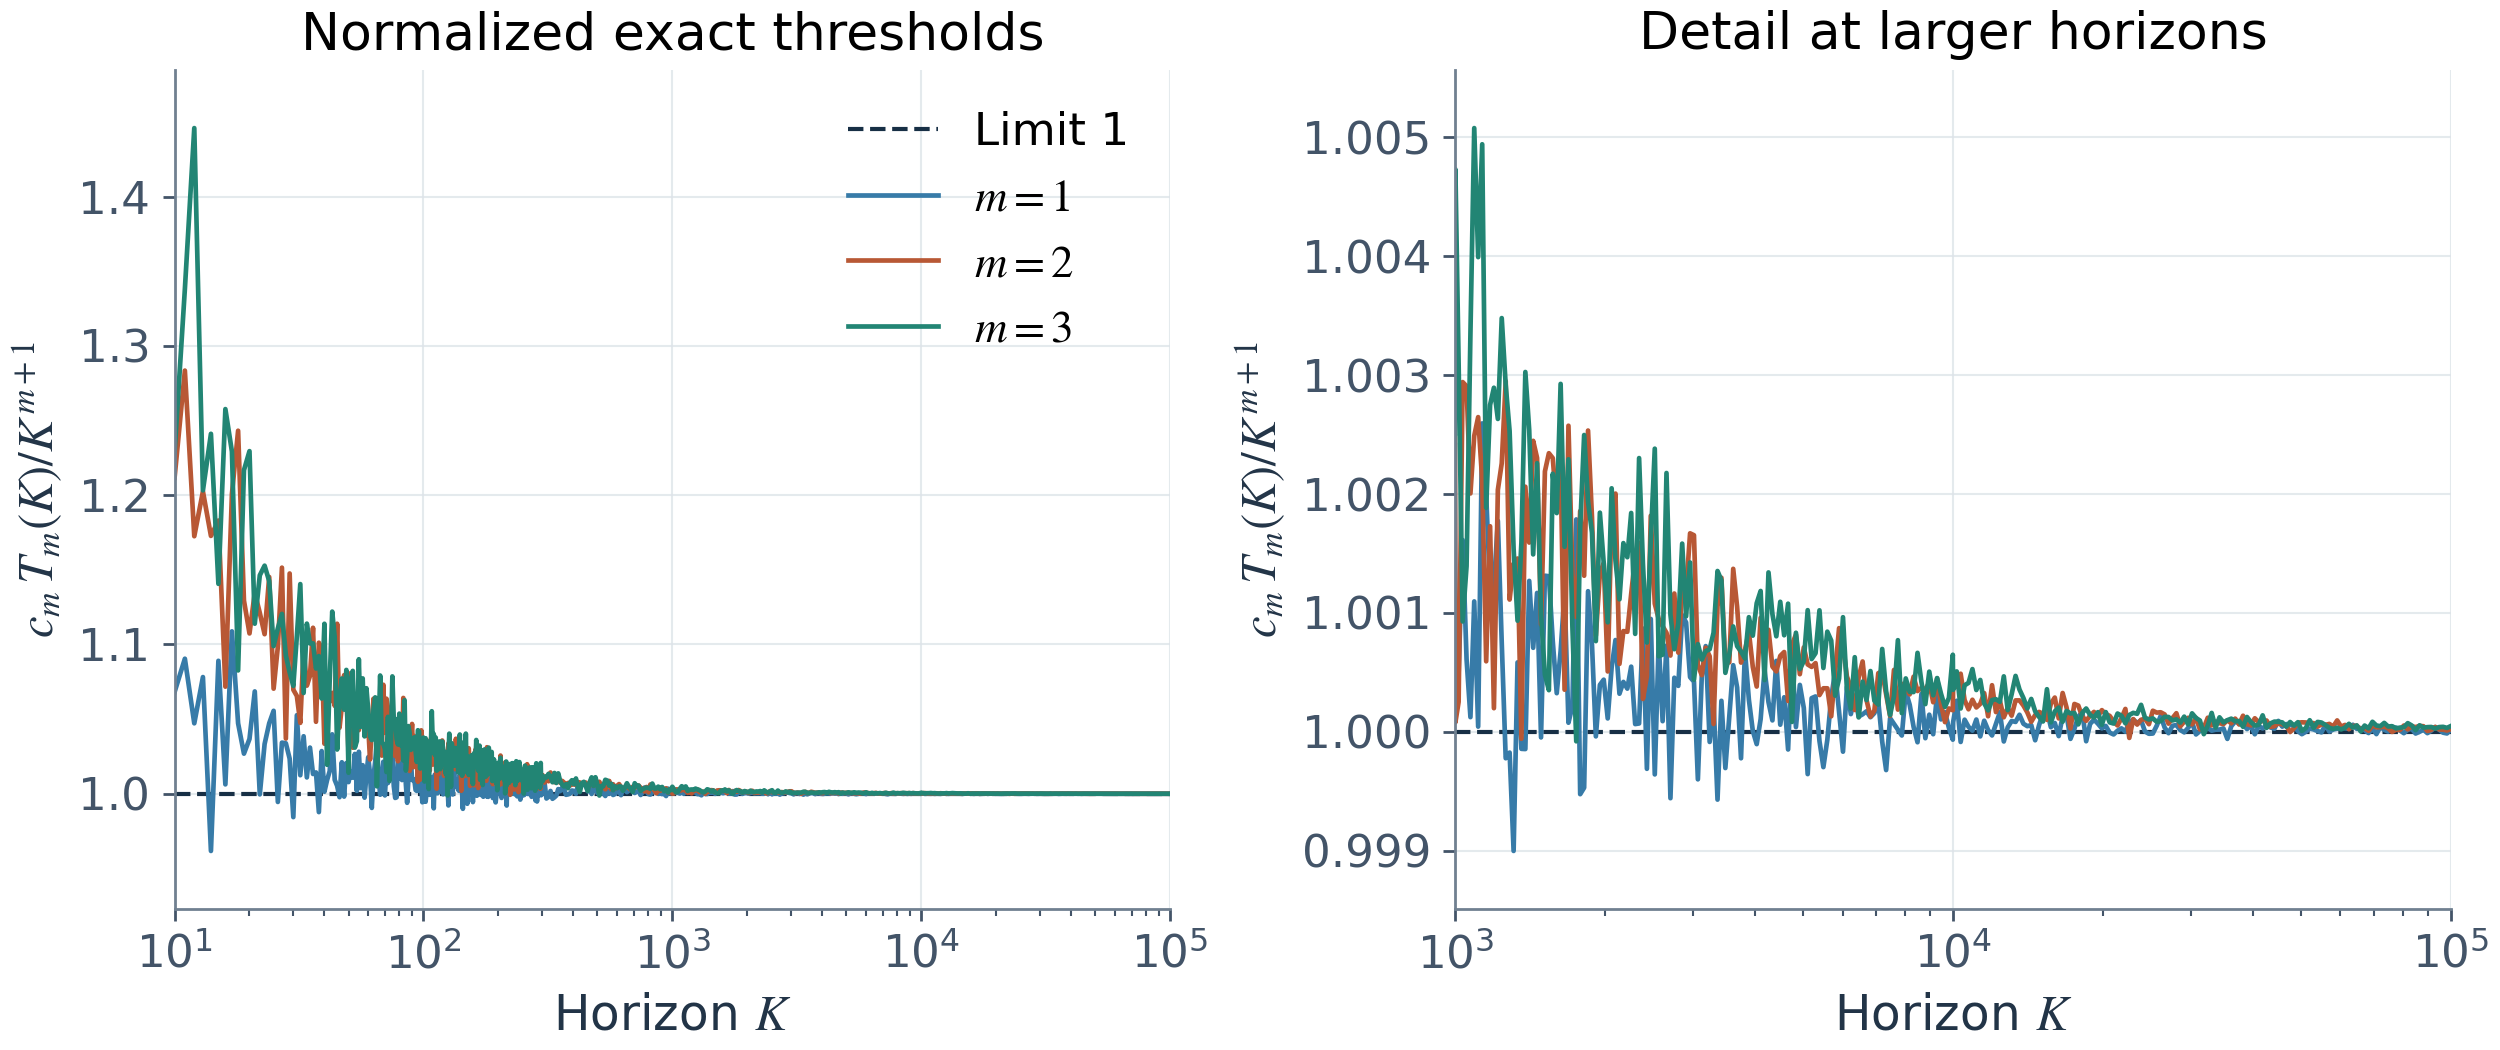
\includegraphics[width=.98\linewidth]{figures/normalized_thresholds.png}
\caption{Normalized thresholds for $m=1,2,3$, calculated by the exact
backward recurrence. The Gamma constants are used only in the
normalization. The irregular excursions illustrate why estimating
a discrete error law requires more than a smooth fitted curve.}
\label{fig:thresholds}
\end{figure}

\subsection{The predicted shapes}

\begin{figure}[tbp]
\centering
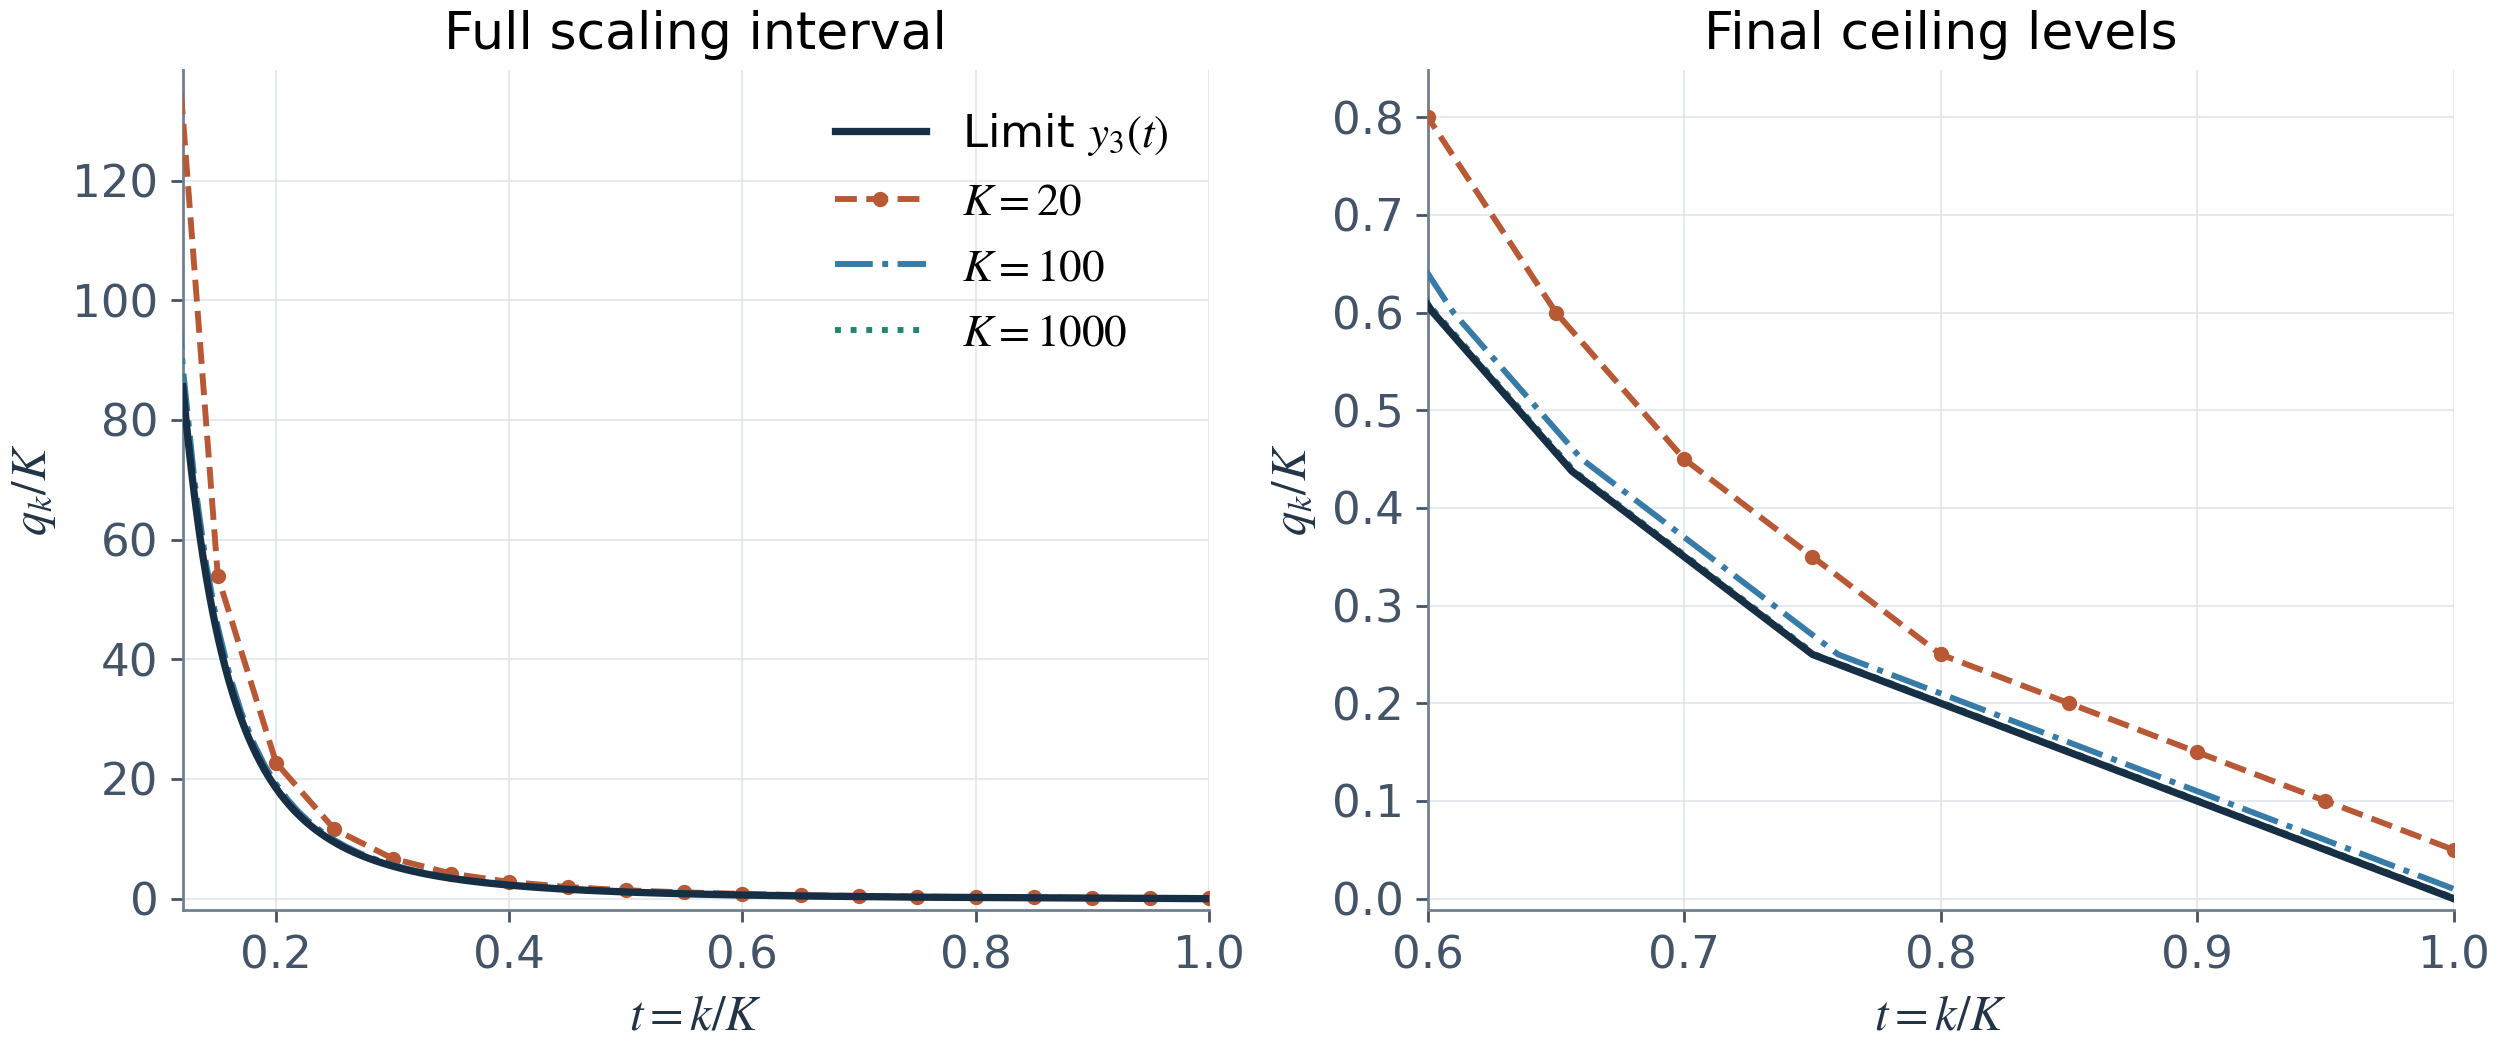
\includegraphics[width=.98\linewidth]{figures/backward_profiles.png}
\caption{The cubic backward quotient profile. Discrete arrays, divided
by their terminal stage $K$, approach the explicit piecewise linear
function $y_3$. The plot stays away from $t=0$, where $y_3$ diverges;
the proof handles that endpoint through weighted tail bounds.}
\label{fig:backward}
\end{figure}

Figure~\ref{fig:backward} directly illustrates the compact convergence
proved in \cref{prop:profile}. Figure~\ref{fig:forward} uses actual
forward trajectories, which were not used to construct the limiting
profile. For the cubic process, the exact stopping indices for initial
values $10^3,10^6,10^9$ are respectively $9,51,287$. The step curves
converge to the continuous weighted profile $F_3$.

\begin{figure}[tbp]
\centering
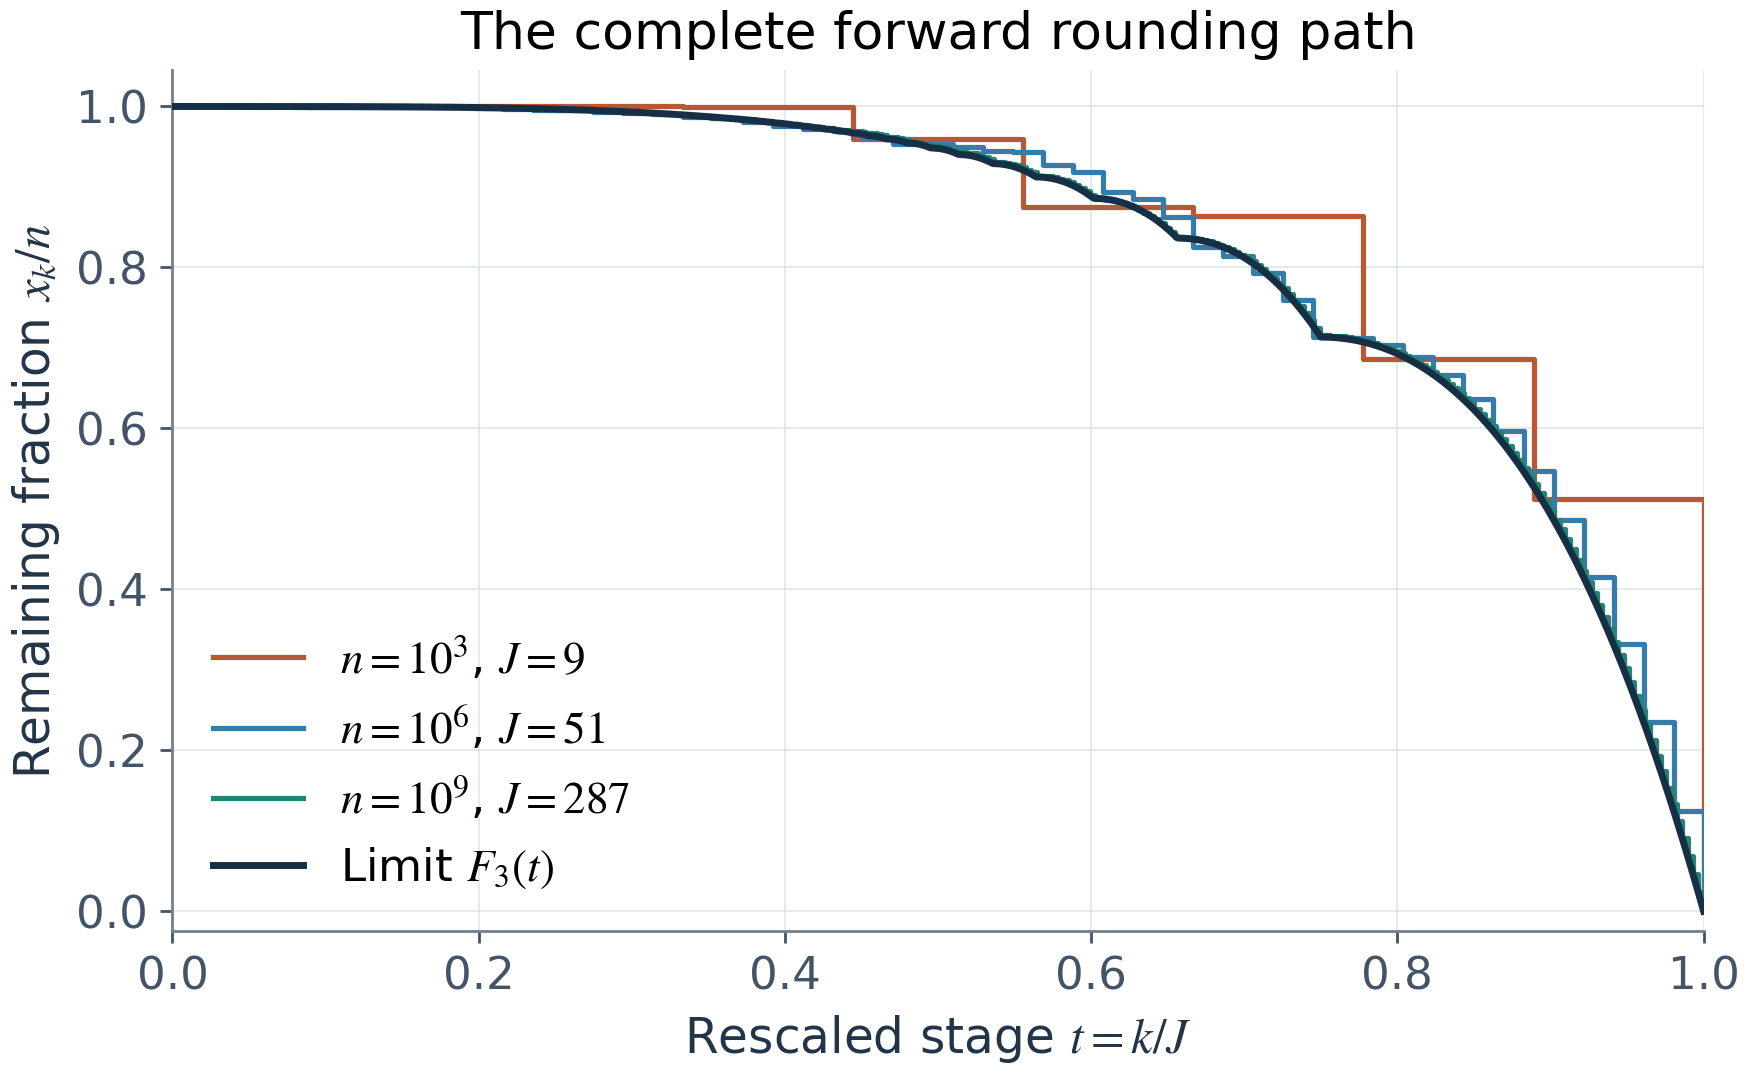
\includegraphics[width=.98\linewidth]{figures/forward_paths.png}
\caption{The fraction of the initial value remaining in three cubic
forward trajectories, with time divided by the exact stopping index.
The limiting curve is $F_3(t)=c_3t^3y_3(t)$. Its continuous value at
$t=0$ is $1$, despite the divergence of the unweighted quotient profile.}
\label{fig:forward}
\end{figure}

\subsection{Certified constant intervals}

\begin{table}[tbp]
\centering
\small
\begin{tabular}{rrrr}
\toprule
$m$ & Lower endpoint & $m\Gamma(m/(m+1))^{m+1}$ & Upper endpoint\\
\midrule
1 & 3.1408077460 & 3.1415926536 & 3.1423781500\\
2 & 4.9642631432 & 4.9659171624 & 4.9675726521\\
3 & 6.7622883375 & 6.7648229810 & 6.7673600538\\
5 & 10.3385883285 & 10.3428938609 & 10.3472038189\\
\bottomrule
\end{tabular}

\caption{Finite-product enclosures from \cref{prop:certificates} at
$j=1000$. The outer decimal endpoints are rounded outward by exact
integer arithmetic, so the displayed intervals retain the enclosure.
The middle column is a numerical evaluation of the exact Gamma formula.}
\label{tab:certificates}
\end{table}

The exact rational numerators and denominators underlying
Table~\ref{tab:certificates} are included in
\begin{quote}\ttfamily
data/constant\_certificates.json
\end{quote}
The table's enclosure is
provided by the theorem and exact endpoint arithmetic. A numerical
comparison of a Gamma evaluation with those intervals is an additional
consistency check, not the basis of their certification.

\subsection{Reproduction and formalization}

The archive includes the LaTeX source, this PDF, the figures, the Python
program, its dependency versions, and recorded data. From the archive's
root directory, the full calculation is reproduced by
\begin{quote}\ttfamily
python reproduce.py
\end{quote}
The exact checks alone require only the Python standard library:
\begin{quote}\ttfamily
python reproduce.py --exact-only --out replay\_exact
\end{quote}
The full replay additionally uses \texttt{mpmath} and
\texttt{matplotlib}; it requires no network access. Compile
\texttt{article.tex} twice with \texttt{pdflatex} to rebuild the PDF.
The README gives query examples, output descriptions, and precision
conventions.

A formalization can be divided at natural mathematical interfaces.
The finite recurrence and survival duality need only integer order,
floor/ceiling inequalities, and finite induction. Rational exponents
admit an exact integer-root specification. The analytic part requires
compactness of uniformly Lipschitz functions on compact intervals,
dominated convergence, the Gamma functional equation, and the beta
integral. The proof isolates the delicate points as reusable lemmas:
the positive drift that selects the terminal solution, the finite
number of ceiling discontinuities on compact intervals, and the final
weighted tail estimate.

No proof-assistant development accompanies this report. The executable
checks are finite computations and are not described as a formal
verification of the real-parameter theorem.


\section{Further research questions}\label{sec:questions}

The leading constant is only the first part of the rounding problem.
The following questions separate plausible next steps from conclusions
already proved. They are proposed research problems; except for the
historical linear question, their open status refers to this report
and the sources inspected, not to an exhaustive classification of the
literature.

\begin{question}[Quantitative threshold errors]\label{q:rates}
For fixed $m>0$, find a usable rate in
\[
 T_m(K)=L_mK^{m+1}+E_m(K).
\]
Which exponents $\delta_m>0$ admit
$E_m(K)=O_m(K^{m+1-\delta_m})$? Can an explicit bound be obtained
uniformly for $m$ in a compact subinterval of $(0,\infty)$?
\end{question}

The proof identifies the correct place to work: make the crossing
times of the discrete quotient increments quantitative, then balance
their accumulated errors against the omitted small-time tail. The
classical $m=1$ estimate in \cref{eq:classical-error} supplies a
benchmark. Compactness alone contains no numerical rate.

\begin{question}[Bounded stopping-time error]\label{q:bounded}
For which $m>0$, if any, does
\[
 \tau_m(n)=(c_mn)^{1/(m+1)}+O_m(1)
\]
hold? In particular, resolve the stronger bounded-error claim for
$m=1$ recorded in A073047.
\end{question}

For pure powers, this is equivalent to
$T_m(K)=L_mK^{m+1}+O_m(K^m)$. One direction follows by inverting the
two neighboring threshold bounds. For the other, evaluate the
stopping-time formula at the first integer of each survival interval,
where the stopping index is $K+1$, and expand the resulting power.
The two equivalent formulations indicate that an error term at the
scale of a single threshold gap is required.

\begin{question}[Signs and fluctuation scales]
Does $T_m(K)-L_mK^{m+1}$ have an eventual sign? What are the natural
scales of its upper and lower envelopes? Does any centered and scaled
version have a limiting distribution along integer horizons?
\end{question}

The selected tabulated horizons have positive errors, while the denser
plotted data include both signs. Neither observation establishes an
eventual-sign theorem. The nonmonotone normalized errors show that a
simple monotonicity argument would need additional structure. Any probabilistic terminology here would describe a
distribution over sampled horizons, not randomness in the recurrence.

\begin{question}[A theory of microscopic schedules]\label{q:schedules}
Classify the limits for regularly varying weights when
$k(w_k/w_{k-1}-1)$ oscillates, has repeated zero values, or follows a
periodic pattern. Which information beyond the regular-variation
index determines the extinction constant and the limiting profile?
\end{question}

The block construction gives a completely solved test family. A
possible next class consists of a fixed periodic pattern of small
relative increments. The ceiling acts before any averaging, so an
effective drift would have to be derived from the individual phases
of that pattern. Establishing such an averaging theorem is a
substantive extension; it is not a consequence of
\cref{thm:weights-main}.

\begin{question}[Stability under sparse exceptional steps]
How many exceptional ratios can be allowed without changing $L_m$?
For example, suppose the local ratio condition holds outside a set
of indices of density zero. Which bounds on the exceptional
increments suffice, and can a sparse set of very large jumps change
the constant?
\end{question}

Finite modifications are already covered. Passing from finitely many
exceptions to a sparse infinite set requires controlling their
combined effect on the quotient increments. Density alone need not
control the size of those effects.

\begin{question}[Moving exponents and singular regimes]
Describe joint limits with $m=m(n)\downarrow0$ or $m=m(n)\to\infty$.
Determine ranges in which the fixed-parameter equivalent remains
uniform and identify any transition scales.
\end{question}

The discontinuity at $m=0$ makes the first question particularly
interesting: positive integer values never vanish when every weight
is exactly $1$. The explicit expansions in
\cref{prop:parameter} describe the constants, but they do not control
the speed of convergence of the underlying discrete process.

\begin{question}[Rates for the full trajectory and loss distribution]
Obtain explicit bounds for
\[
 \sup_{0\leq t\leq1}|X_n(t)-F_m(t)|
\]
and for convergence of the loss measures in
\cref{cor:losses}. Can one derive asymptotics for individual moments
or quantiles of the loss-time distribution with a controlled error?
\end{question}

The limiting density is explicit on each increment regime. It permits
certified computation of limiting observables using finite sums and
an integrable tail. Rates for the finite process again depend on
discrete crossing errors rather than solely on the Gamma constant.

\begin{question}[Sieve and game interpretations for higher powers]
Is there a natural sieve or solitaire model whose survival thresholds
are $T_m(K)$ for integer $m\geq2$? Can such a model explain the
Gamma product combinatorially or connect the threshold gaps to an
existing family of integer sequences?
\end{question}

The ordinary case has the Tchoukaillon interpretation. A higher-power
model could expose monotonicity, congruence, or conservation
properties not apparent in the floor recurrence. Any proposed model
should first be proved equivalent to the exact backward recurrence,
including its initial conditions.

\begin{question}[Faster exact algorithms and formal verification]
Can long consecutive ranges with a constant quotient increment be
skipped in a provably correct exact algorithm? Can the general
real-parameter theorem be formalized with a reusable library lemma
for monotone discontinuous drift limits?
\end{question}

The present algorithm takes one arithmetic step per stage. The
limiting piecewise linear structure suggests acceleration, but the
exact locations of discrete transitions must be certified before
steps can be skipped. For formalization, a useful first milestone is
the exact survival duality and rational-exponent algorithm, followed
by the compactness and endpoint-selection lemmas.

\subsection{A practical order for continuing the work}

The most direct continuation is a quantitative crossing-time analysis
for the pure power family. In parallel, a periodic-ratio model can
test how the constant changes when the local smoothness condition is
relaxed. These two directions address the principal limitations of
the present theorem: the absence of a finite error bound, and the
dependence on the microscopic schedule.

\appendix
\section{Proof dependencies and source audit}\label{app:audit}

\subsection{Logical dependencies}

The extinction proof proceeds through five independently checkable
steps:
\begin{enumerate}
\item Exact stagewise survival duality gives the backward ceiling
recurrence and the inverse threshold relation.
\item The integer increment bound and weighted rounding-error bound
give compactness and force positive terminal drift.
\item Strict monotonicity of $my(t)/t$ controls the ceiling
discontinuities, yielding a rigorous limit equation.
\item Solving its increment regimes gives the finite product;
the beta integral evaluates its asymptotic constant.
\item A telescoping estimate controls the entire omitted initial
part, allowing the two limits to be taken in the correct order.
\end{enumerate}
The smooth-weight theorem reuses these steps after proving the local
ratio and tail-sum consequences of its hypothesis. The forward-path
theorem follows from a second use of the exact stagewise duality.
No numerical estimate is an input to any of these proofs.

Two independent mathematical reviews checked the ceiling passage,
initial-value convention, smooth-weight tail, inversion, profile
endpoint argument, and block counterexample. The exact finite
verification was generated by a separate implementation. These
reviews improve confidence but are not a substitute for peer review
or formal verification.

\subsection{Sources reviewed and scope of the novelty statement}

The principal source records are the OEIS definitions and conjectures
for A073047, A082527, and A082528; the classical threshold entry
A002491; Erd\H{o}s and Jabotinsky's original sieve paper; the
Broline--Loeb preprint and the criticism attributed to Knuth in the
threshold entry; Brown's exposition; Leh\'ericy's 2023 proof for a
different generalized rounding rule; and Li's 2026 Tchoukaillon
preprint. The bibliography provides direct links.

Targeted searches combined the exact sequence identifiers with
power-rounding, asymptotic, Gamma, generalized sieve, and the
classical authors' names. Searches within ProveIt used the exact
sequence identifiers and Tchoukaillon-related terms. No matching
real-power theorem or formula for $c_m$ was found in that review.
This statement is intentionally bounded by the sources and search
scope. A conjectural label remaining on an OEIS entry does not prove
that no proof exists elsewhere.

The result should therefore be described precisely: this report
supplies a complete proof of the real-parameter conjecture as
recorded in A082528, identifies the square and cube constants, and
proves the stated extensions. It makes no claim to have newly
discovered the linear $\pi$ law or the general increment-regime
method. The numerical and symbolic evidence in the archive is
reproducible and separately labeled.

\section{Suggested OEIS update text}\label{app:oeis}

The following concise mathematical statements are suitable for
review before any submission. They have not been posted to OEIS.

\paragraph{For A082527.}
The conjectured asymptotic constant is
\[
c=2\Gamma(2/3)^3=4.965917162430455473\ldots.
\]
Thus $a(n)\asym(2\Gamma(2/3)^3n)^{1/3}$.
This is the $m=2$ case of the power-rounding extinction theorem.

\paragraph{For A082528.}
For every fixed real $m>0$, if $x_1=n$ and
$x_k=k^m\lfloor x_{k-1}/k^m\rfloor$, the first zero satisfies
\[
 a(n,m)\asym
 \left(m\Gamma\!\left(\frac{m}{m+1}\right)^{m+1}n\right)^{1/(m+1)}.
\]
In particular, the cubic constant is
$3\Gamma(3/4)^4=6.764822981008760234\ldots$.
A proof is given by the backward survival thresholds and their
piecewise linear scaling limit.

\paragraph{For the linear cross-reference.}
The $m=1$ specialization is the classical leading equivalent
$a(n)\asym\sqrt{\pi n}$. It does not establish the stronger $O(1)$
error term in A073047.

\clearpage

\begin{thebibliography}{99}
\raggedright
\addcontentsline{toc}{section}{References}

\bibitem{oeis-linear}
B. Cloitre and contributors,
\emph{A073047: Least $k$ such that $x(k)=0$ where $x(1)=n$ and
$x(k)=k\lfloor x(k-1)/k\rfloor$},
The On-Line Encyclopedia of Integer Sequences.
Entry introduced 31 August 2002; revised description 3 May 2003.
\url{https://oeis.org/A073047}.

\bibitem{oeis-square}
B. Cloitre and contributors,
\emph{A082527: Repeated rounding down to multiples of $k^2$},
The On-Line Encyclopedia of Integer Sequences, 30 April 2003.
\url{https://oeis.org/A082527}.

\bibitem{oeis-cube}
B. Cloitre and contributors,
\emph{A082528: Repeated rounding down to multiples of $k^3$},
The On-Line Encyclopedia of Integer Sequences, 30 April 2003.
Includes the conjecture for general real $m>0$.
\url{https://oeis.org/A082528}.

\bibitem{oeis-threshold}
N. J. A. Sloane and contributors,
\emph{A002491: Smallest number of stones in Tchoukaillon solitaire
that make use of the $n$th hole},
The On-Line Encyclopedia of Integer Sequences.
Includes the upward-rounding description and D. E. Knuth's comment
of 8 June 2021, recorded 9 June 2021, on the claimed sharp error bound.
\url{https://oeis.org/A002491}.

\bibitem{erdos-jabotinsky}
P. Erd\H{o}s and E. Jabotinsky,
\emph{On sequences of integers generated by a sieving process. I, II},
Proceedings of the Koninklijke Nederlandse Akademie van Wetenschappen,
Series A \textbf{61} = Indagationes Mathematicae \textbf{20} (1958),
115--123 and 124--128. The linear rounding asymptotic and the
$O(K^{4/3})$ estimate are in Part I, Section 2.
\url{https://www.renyi.hu/~p_erdos/1958-08.pdf};
\url{https://www.renyi.hu/~p_erdos/1958-09.pdf}.

\bibitem{broline-loeb}
D. M. Broline and D. E. Loeb,
\emph{The combinatorics of Mancala-type games: Ayo, Tchoukaillon,
and $1/\pi$}, 1995, arXiv:math/9502225.
\url{https://arxiv.org/abs/math/9502225}.
For the error-term issue discussed here, see the attributed comment
in \cite{oeis-threshold}.

\bibitem{brown}
K. S. Brown, \emph{Rounding up to $\pi$}, MathPages.
\url{https://www.mathpages.com/home/kmath001/kmath001.htm}.

\bibitem{lehericy}
T. Leh\'ericy,
answer to r.e.s., \emph{How to prove this recurrence relation for
generalized ``rounding up to $\pi$''?}, Mathematics Stack Exchange,
24 May 2023, revised 25 May 2023.
\url{https://math.stackexchange.com/a/4705436}.

\bibitem{li}
S. Li, \emph{Asymptotics of the Tchoukaillon array and a conjecture
of Beluhov}, arXiv:2608.17517v1, 18 August 2026.
\url{https://arxiv.org/abs/2608.17517}.

\bibitem{dlmf}
F. W. J. Olver et al., editors,
\emph{NIST Digital Library of Mathematical Functions},
Chapter 5, especially Sections 5.7 and 5.15.
\url{https://dlmf.nist.gov/5.7};
\url{https://dlmf.nist.gov/5.15}.

% Added by the ProveIt write phase (batch 110): cited by Part III.
\bibitem{averaging}
M. Fe\v{c}kan, J. Pa\v{c}uta, M. Posp\'i\v{s}il, and P. Vidli\v{c}ka,
\emph{Averaging methods for piecewise-smooth ordinary differential equations},
AIMS Mathematics \textbf{4}(5) (2019), 1466--1487.
\url{https://doi.org/10.3934/math.2019.5.1466}.
Background on discontinuous averaging, not an invoked theorem for
the present discrete process (Part~III).

\bibitem{proveit}
V. Reshetnikov and contributors,
\emph{ProveIt}, GitHub repository.
\url{https://github.com/VladimirReshetnikov/ProveIt}.
Inspected source snapshot:
\texttt{ce37e13f4aa16819c87c3ccc611362d15758f2ac}.

\end{thebibliography}

